\scanpage{24}\mspage{23}
Mais maintenant, on est ennuyé, car $]a,b[$ n'a plus envie d'être ouvert !

\deleted{\unsure{ici|on}} On peut bien sûr prendre la topologie borne sup. des deux, ayant comme base d'ouverts

\[
\begin{aligned}
 \mathcal L_{<a},\,\mathcal L_{>a},\quad &]a,b[ && (a<b)\\
 \complement \mathcal L_{\deleted{\unsure{\leq|>}}\geq a},\,\complement \mathcal L_{\leq a},\quad &[a,b] && (a<b)
\end{aligned}
\]

\deleted{De sorte que $]a,b[$ \unsure{est|est un}} \deleted{Sera-t-il vrai, si $a\unsure{\nless|\leq|<}b$, et} \deleted{Mais} \deleted{$b$ n'est pas plus grand élément, que}

Aura-t-on \deleted{$b\in [a,b$}
\[
\begin{aligned}
 \overline{]a,b[}&=[a,b]\quad ?\\
 \overline{\mathcal L_{<a}}&=\mathcal L_{\leq a}\quad ?\quad \text{(si $a$ \deleted{\unsure{n'|est}} n'est pas plus petit élément\unsure{—|)}} \quad \inserted{(a\ne\unsure{o|0}_{L})}\\
 \overline{\mathcal L_{>a}}&=\mathcal L_{\geq a}\quad ?\quad \text{(si $a$ n'est pas plus grand élément ?)}
\end{aligned}
\]

\figure{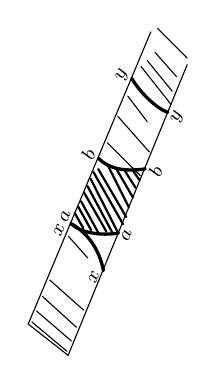
\begin{tikzpicture}[rotate=67,x=.84cm,y=.84cm,line cap=round,line join=round,every node/.style={transform shape,inner sep=1pt,font=\scriptsize}]\draw (.20,.74)--(4.99,.76) (0,0)--(4.75,.06);\draw (0,0)--(.20,.74);\draw[thin] (.05,.04)--(.25,.70) (.22,.04)--(.43,.70) (.44,.05)--(.67,.71) (.72,.05)--(.94,.70) (1.47,.30)--(1.66,.70) (2.93,.06)--(3.19,.71) (3.31,.07)--(3.62,.72) (3.72,.28)--(3.96,.70) (4.10,.05)--(4.45,.69) (4.29,.11)--(4.57,.64) (4.52,.14)--(4.73,.58) (4.84,.10)--(5.08,.69);\draw[very thick] (1.39,.01) .. controls (1.64,.18) and (1.82,.43) .. (1.85,.74) (2.00,.02) .. controls (1.85,.26) and (1.78,.55) .. (1.85,.74) (3.05,.03) .. controls (2.88,.31) and (2.84,.54) .. (2.92,.74) (3.97,.05) .. controls (3.96,.23) and (4.08,.55) .. (4.23,.75);\draw[thick] (1.86,.54)--(2.02,.75) (1.88,.42)--(2.13,.74) (1.89,.31)--(2.22,.73) (1.95,.20)--(2.36,.74) (1.97,.11)--(2.47,.73) (2.01,.04)--(2.59,.73) (2.15,.01)--(2.70,.73) (2.27,.01)--(2.77,.68) (2.42,.03)--(2.87,.56) (2.58,.03)--(2.88,.43) (2.73,.05)--(2.91,.31) (2.86,.04)--(2.96,.20);\node[above] at (1.69,.75) {$x$};\node[above] at (1.92,.75) {$a$};\node[above] at (2.91,.75) {$b$};\node[above] at (4.22,.76) {$y$};\node[left] at (1.38,.10) {$x$};\node[below] at (2.01,.01) {$a$};\node[below] at (3.07,.02) {$b$};\node[below] at (3.96,.03) {$y$};\end{tikzpicture}}
\deleted{\unsure{Donc|D'où}} On est ramené, dans le premier cas, à prouver (p. ex.) $a\in\overline{]a,b[}$, et pour ceci, \inserted{il suffit de voir} \deleted{On} que tte ouvert ``élémentaire'' qui contient $a$, contient un $]a,\varepsilon[$, avec $a<\varepsilon<b$. Mais c'est faux déjà pour un ens. de lieux associé à une ficelle topologique, \deleted{\unsure{en}} [prendre ouvert él. $\complement[x,y]$\unsure{—|.}

% slanted
\margin{Il faut avoir que $a\in\complement[x,y]$ mais $]a,b[\,\subset [x,y]$}

% pale vertical watermark
\rotatebox{90}{\textsc{\unsure{Strong Extra}}}
